\chapter{Le traitement d'images}
\label{chap-images}
\chapteroverview{Une image numérique est un tableau de nombres : la modifier revient donc à calculer avec ces nombres. Ce chapitre présente des méthodes simples pour stocker les images, réduire leur bruit, détecter les contours et manipuler les couleurs. Chaque exemple relie un effet visible à une formule explicite et précise ce que l'opération conserve ou fait perdre.}

\section{Pixels et niveaux de gris}
Une image en niveaux de gris ayant $n$ lignes et $p$ colonnes contient $np$ \emph{pixels}. Dans la représentation sur huit bits étudiée ici, chaque pixel contient un entier compris entre $0$ et $255=2^8-1$. Zéro est affiché en noir, 255 en blanc et les valeurs intermédiaires en nuances de gris. D'autres profondeurs de codage et des représentations en nombres flottants sont également utilisées.

La fleur de la figure~\ref{fig-section1-original-zoom} comporte $256\times256=65\,536$ pixels. L'agrandissement montre un carré de $5\times5$ pixels : chaque nuance affichée correspond à l'un des nombres du tableau. Une photographie peut contenir des millions de pixels, mais le principe reste le même.
\myfigure{\imageL{section1-original-zoom}}
{Une image et l'agrandissement d'un carré de $5\times5$ valeurs de pixels.}{fig-section1-original-zoom}

\section{Stocker une image}
\subsection{Écriture binaire et unités de stockage}
L'écriture binaire d'un entier s'obtient en le décomposant en puissances de deux. Par exemple,
\[
 179=2^7+2^5+2^4+2^1+2^0
    =\underbrace{(10110011)_2}_{\text{écriture binaire}}.
\]
En allant de $2^7$ à $2^0$, on inscrit un bit égal à un si la puissance correspondante apparaît, et zéro sinon. Huit bits suffisent pour représenter tous les entiers de 0 à 255.

Une image en niveaux de gris sur huit bits non compressée demande donc $8np$ bits, soit $np$ \emph{octets}, pour les valeurs des pixels. La fleur de $256\times256$ pixels occupe
\[
 256\times256\times8=524\,288\ \text{bits}
       =65\,536\ \text{octets}.
\]
Cela représente $65{,}536$ ko en unités décimales, ou $64$ Kio en unités binaires : un ko vaut $1000$ octets, tandis qu'un Kio vaut $1024$ octets. À titre de comparaison, une image de $240\times240$ pixels demanderait $57\,600$ octets, soit $56{,}25$ Kio. Les en-têtes de fichier et les métadonnées s'ajoutent à ces volumes.

\subsection{Sous-échantillonnage}
Réduire le nombre de pixels diminue le volume de stockage. Conserver une ligne sur quatre et une colonne sur quatre divise ce nombre par $4^2=16$, lorsque les deux dimensions sont divisibles par quatre. La figure~\ref{fig-section2-subsample} montre des grilles de plus en plus grossières.
\myfigure{\imageTri{section2-subsample-4}{section2-subsample-8}{section2-subsample-16}
{Une ligne/colonne sur 4}{Une ligne/colonne sur 8}{Une ligne/colonne sur 16}}
{Sous-échantillonnage sur des grilles de plus en plus grossières.}{fig-section2-subsample}

Supprimer des lignes et des colonnes peut effacer des détails et créer de faux motifs : c'est le phénomène de \emph{repliement spectral}, ou aliasing. En pratique, on lisse généralement l'image avant de réduire sa fréquence d'échantillonnage. Le chapitre suivant explique la raison mathématique de cette précaution.

\subsection{Quantification}
On peut aussi réduire le stockage en diminuant le nombre de valeurs possibles par pixel. Pour ne conserver que quatre niveaux, on remplace une valeur $a\in\{0,\ldots,255\}$ par
\[
 q(a)=\left\lfloor\frac a{64}\right\rfloor\in\{0,1,2,3\}.
\]
Ainsi, les valeurs de $0$ à $63$ deviennent $0$, celles de $64$ à $127$ deviennent $1$, celles de $128$ à $191$ deviennent $2$, et celles de $192$ à $255$ deviennent $3$. Affichés sur une échelle du noir au blanc, ces indices correspondent respectivement au noir, au gris foncé, au gris clair et au blanc ; on peut les restituer par les valeurs $85q(a)$.

Quatre indices demandent deux bits au lieu de huit : le gain est donc d'un facteur quatre si ces indices sont effectivement regroupés dans le fichier. Les conserver dans des emplacements de huit bits ne produirait pas ce gain. La figure~\ref{fig-section3-quantize} compare quatre et seize niveaux.
\myfigure{\imageDuo{section3-quantize-4}{section3-quantize-16}{4 niveaux de gris}{16 niveaux de gris}}
{Quantification avec deux nombres de niveaux différents.}{fig-section3-quantize}

La quantification est généralement irréversible : plusieurs valeurs initiales partagent le même indice. La compression sans perte conserve au contraire toutes les valeurs tout en exploitant les redondances de leur représentation. JPEG 2000 utilise les ondelettes et propose des modes avec et sans perte ; c'est un exemple de codec, et non une méthode universellement meilleure pour toute image et tout critère.\footnote{\url{https://jpeg.org/jpeg2000/}}

\section{Réduire le bruit}
\subsection{Moyenne locale}
Le bruit produit des fluctuations indésirables des valeurs des pixels. Il est particulièrement visible dans les photographies prises en faible lumière, mais sa distribution dépend du capteur et du procédé d'acquisition. Une méthode simple de débruitage remplace chaque pixel par la moyenne d'une fenêtre autour de lui.

Pour le voisinage de $3\times3$ pixels de la figure~\ref{fig-section5-moyenne-numbers}, on remplace la valeur centrale $a$ par
\[
 \frac{a+b+c+d+e+f+g+h+i}{9}.
\]
Les valeurs affichées donnent
\[
 \frac{190+192+79+54+47+153+203+189+166}{9}
       =\frac{1273}{9}\simeq141{,}44.
\]
\myfigure{\imageM{section5-moyenne-numbers}}
{Un voisinage de $3\times3$ pixels pour le calcul d'une moyenne ou d'une médiane locale.}{fig-section5-moyenne-numbers}

Toutes les moyennes doivent être calculées à partir de la même image d'entrée. Modifier les pixels sur place, puis réutiliser ces nouvelles valeurs, définit un autre filtre. Au bord de l'image, il faut également choisir une convention, par exemple prolonger l'image par réflexion ou restreindre la fenêtre en renormalisant ses poids.

Pourquoi la moyenne est-elle utile ? Si un signal localement constant est perturbé par un bruit indépendant, centré et de variance $\sigma^2$, la moyenne de $m$ pixels a une variance de bruit égale à $\sigma^2/m$. Près d'un contour, le signal n'est cependant pas constant : la moyenne mélange des régions distinctes et introduit du flou. Agrandir la fenêtre réduit davantage le bruit, mais efface plus de détails.
\myfigure{\begin{tabular}{@{}c@{\hspace{2mm}}c@{\hspace{2mm}}c@{\hspace{2mm}}c@{}}
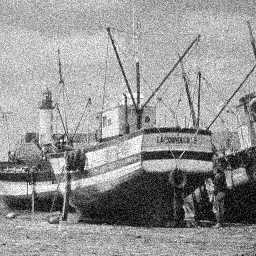
\includegraphics[width=.23\linewidth]{section5-noisy}&
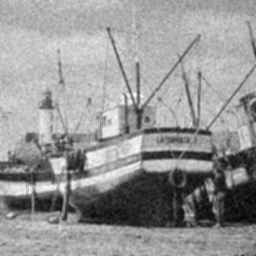
\includegraphics[width=.23\linewidth]{section5-moyenne-1}&
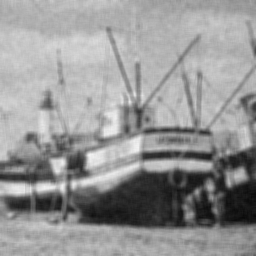
\includegraphics[width=.23\linewidth]{section5-moyenne-2}&
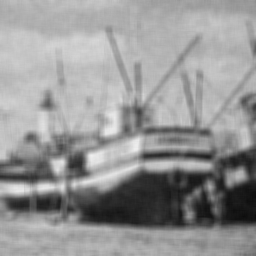
\includegraphics[width=.23\linewidth]{section5-moyenne-3}\\
Image bruitée&Moyenne $3\times3$&Moyenne $5\times5$&Moyenne $7\times7$
\end{tabular}}{La moyenne locale réduit le bruit, mais rend les contours plus flous lorsque la fenêtre grandit.}{fig-section5-moyenne}

\subsection{Médiane locale}
La \emph{médiane} d'un nombre impair de valeurs est la valeur centrale après leur classement. Les neuf valeurs précédentes, dans l'ordre croissant, sont
\[
 47,54,79,153,166,189,190,192,203.
\]
Leur médiane est donc $166$. Le filtre médian remplace chaque pixel par la médiane de son voisinage dans l'image d'entrée.

La médiane résiste aux valeurs extrêmes isolées et préserve souvent mieux les transitions nettes que la moyenne. Elle est particulièrement utile contre le bruit impulsionnel, mais n'est pas systématiquement meilleure pour toute image et tout modèle de bruit. De grandes fenêtres peuvent effacer les objets fins et les petits détails. La figure~\ref{fig-section6-mediane} illustre ce compromis.
\myfigure{\begin{tabular}{@{}c@{\hspace{2mm}}c@{\hspace{2mm}}c@{\hspace{2mm}}c@{}}
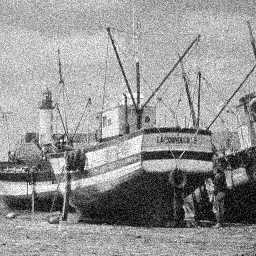
\includegraphics[width=.23\linewidth]{section5-noisy}&
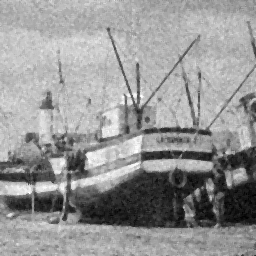
\includegraphics[width=.23\linewidth]{section6-mediane-1}&
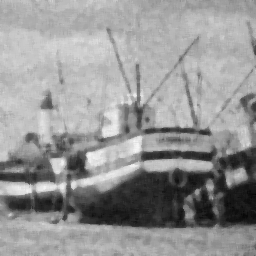
\includegraphics[width=.23\linewidth]{section6-mediane-2}&
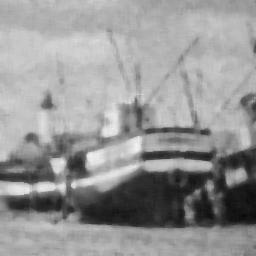
\includegraphics[width=.23\linewidth]{section6-mediane-3}\\
Image bruitée&Médiane $3\times3$&Médiane $5\times5$&Médiane $7\times7$
\end{tabular}}{Filtrage médian avec une fenêtre de taille croissante.}{fig-section6-mediane}

\section{Détecter les contours}
Les contours sont des zones où les valeurs des pixels varient rapidement, par exemple à la frontière entre un objet sombre et un fond clair. Un détecteur simple compare les voisins situés de part et d'autre d'un pixel.
\myfigure{\imageM{section7-contours-numbers}}
{Le pixel central $a$ et ses voisins gauche, supérieur, droit et inférieur $b,c,d,e$.}{fig-section7-contours-numbers}

Avec la disposition de la figure~\ref{fig-section7-contours-numbers}, on définit
\[
 \ell=\sqrt{(b-d)^2+(c-e)^2}.
\]
Pour un pas spatial égal à un pixel, $\ell/2$ est la norme du gradient estimé par différences centrées. Les valeurs de la figure donnent
\[
 \ell=\sqrt{(192-153)^2+(54-189)^2}
      =\sqrt{19\,746}\simeq140{,}52.
\]
On a $\ell=0$ exactement lorsque $b=d$ et $c=e$. Cela n'implique pas que les cinq valeurs soient égales : le détecteur peut manquer certaines oscillations fines. Une grande valeur indique une variation locale importante, due à un contour, à une texture ou au bruit.

Pour l'affichage, on tronque la valeur à $\min(\ell,255)$ puis on l'arrondit. Le minimum est nécessaire car $\ell$ peut dépasser 255. La figure~\ref{fig-section7-contours} affiche les fortes réponses en blanc. Débruiter avant de dériver peut être utile, car les différences amplifient aussi le bruit.
\myfigure{\imageDuo{section7-image}{section7-contours}{Image d'origine}{Réponse de contour $\ell$}}
{Détection des contours par différences entre voisins opposés.}{fig-section7-contours}

\section{Images en couleur}
\subsection{Canaux RVB et synthèse additive}
Une image RVB comporte trois canaux, représentant le rouge, le vert et le bleu. Ce sont des tableaux distincts, mais ils ne sont généralement \emph{pas statistiquement indépendants}. Dans une représentation sur huit bits par canal, un pixel est un triplet $(r,v,b)\in\{0,\ldots,255\}^3$ et demande 24 bits avant compression.

Les valeurs $(255,0,0)$, $(0,255,0)$ et $(0,0,255)$ donnent respectivement du rouge, du vert et du bleu. Le mélange de lumières émises obéit à la synthèse \emph{additive} : rouge et vert, $(255,255,0)$, donnent du jaune ; rouge et bleu, $(255,0,255)$, donnent du magenta. Le blanc correspond à $(255,255,255)$ et le noir à $(0,0,0)$.
\myfigure{\imageDuo{section8-image}{section8-luminance}{Image en couleur}{Moyenne des canaux}}
{Une image en couleur et une représentation en niveaux de gris.}{fig-luminance}
\myfigure{\imageTri{section8-rouge}{section8-vert}{section8-bleu}{Canal rouge}{Canal vert}{Canal bleu}}
{Les trois canaux RVB affichés dans leurs couleurs respectives.}{fig-canaux-coul}
\myfigure{\imageDuo{section8-synthese-additive}{section8-synthese-soustractive}{Synthèse additive}{Synthèse soustractive}}
{Modèles idéalisés des synthèses additive et soustractive.}{fig-section8-synthese}

\subsection{Canaux CMJ et synthèse soustractive}
Une représentation complémentaire idéalisée utilise le cyan, le magenta et le jaune :
\[
 c=255-r,\qquad m=255-v,\qquad j=255-b.
\]
Par exemple, le bleu $(r,v,b)=(0,0,255)$ correspond à $(c,m,j)=(255,255,0)$. Ces variables décrivent l'action \emph{soustractive} de pigments idéaux sur la lumière blanche : le cyan absorbe le rouge, le magenta absorbe le vert et le jaune absorbe le bleu.
\myfigure{\imageTri{section8-cyan}{section8-magenta}{section8-jaune}{Canal cyan}{Canal magenta}{Canal jaune}}
{Les canaux complémentaires CMJ, représentés sur fond blanc.}{fig-canaux-cmj}

Les imprimantes réelles utilisent des conversions dépendant du matériel, généralement avec un canal noir supplémentaire (CMJN). Un écran émet toujours de la lumière RVB : les données CMJ doivent donc être converties pour y être affichées. Ni les primaires d'un écran donné ni les encres d'une imprimante donnée ne reproduisent toutes les couleurs visibles.

\section{Modifier la luminosité et le contraste}
\subsection{Une intensité en niveaux de gris}
Une manière simple de calculer une image en niveaux de gris consiste à moyenner les trois canaux :
\[
 a=\frac{r+v+b}{3}.
\]
C'est l'intensité employée dans les exemples élémentaires de ce chapitre. Ce n'est pas la \emph{luminance} physique, qui pondère des composantes lumineuses linéaires selon la sensibilité visuelle. La moyenne arithmétique de valeurs RVB codées ne mesure donc pas de manière calibrée la lumière émise.\footnote{Pour la définition de la luminance relative en sRGB, voir \url{https://www.w3.org/TR/WCAG22/\#dfn-relative-luminance}.}

\subsection{Transformations ponctuelles en niveaux de gris}
Remplacer $a$ par $255-a$ échange le noir et le blanc et produit un négatif. Pour assombrir une image, on utilise $a\mapsto a^2/255$ ; pour l'éclaircir, on utilise $a\mapsto\sqrt{255a}$. Ces deux applications conservent l'intervalle $[0,255]$.
\myfigure{\imageTri{section4-negatif}{section4-square}{section4-sqrt}{Négatif}{Carré : plus sombre}{Racine : plus clair}}
{Trois transformations ponctuelles de l'intensité en niveaux de gris.}{fig-section4-square}

Les fonctions carré et racine carrée sont réciproques sur l'intervalle réel. Après arrondi à des valeurs de pixels entières, elles ne se compensent plus nécessairement de façon exacte. Elles se généralisent par la transformation de puissance
\[
 \widetilde a=255\left(\frac a{255}\right)^\gamma,
 \qquad \gamma>0,
\]
avec $\widetilde a=0$ pour $a=0$. Pour $0<a<255$, l'image est éclaircie lorsque $\gamma<1$ et assombrie lorsque $\gamma>1$. Les cas $\gamma=1/2$ et $\gamma=2$ correspondent respectivement à la racine carrée et au carré ; $\gamma=1$ laisse les valeurs inchangées.

\subsection{Une transformation en couleur}
Appliquer des modifications sans lien aux trois canaux peut altérer fortement les couleurs. Une solution élémentaire consiste à modifier l'intensité moyenne $a$ tout en conservant le résidu $(r-a,v-a,b-a)$. On pose
\[
 \begin{aligned}
 \widetilde r&=\operatorname{clip}(r+\widetilde a-a),\\
 \widetilde v&=\operatorname{clip}(v+\widetilde a-a),\\
 \widetilde b&=\operatorname{clip}(b+\widetilde a-a),
 \end{aligned}
 \qquad \operatorname{clip}(u)=\max(0,\min(255,u)).
\]
Sans troncature, la nouvelle moyenne vaut $\widetilde a$ et les différences entre canaux sont conservées. La troncature peut modifier ces deux propriétés ; cette construction ne garantit donc pas une conservation exacte de la teinte ou de la saturation perçues. Les valeurs ne sont arrondies qu'à la fin du calcul.
\myfigure{\begin{tabular}{@{}c@{\hspace{1mm}}c@{\hspace{1mm}}c@{\hspace{1mm}}c@{\hspace{1mm}}c@{\hspace{1mm}}c@{}}
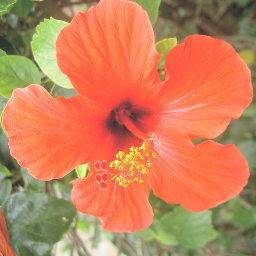
\includegraphics[width=.15\linewidth]{section4-constrast-1}&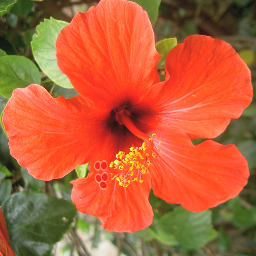
\includegraphics[width=.15\linewidth]{section4-constrast-2}&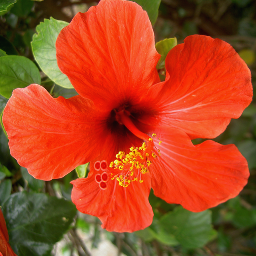
\includegraphics[width=.15\linewidth]{section4-constrast-3}&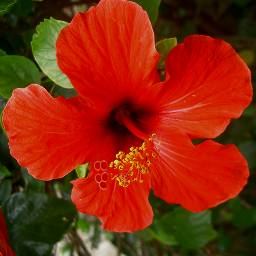
\includegraphics[width=.15\linewidth]{section4-constrast-4}&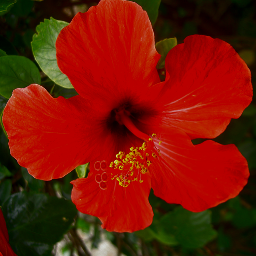
\includegraphics[width=.15\linewidth]{section4-constrast-5}&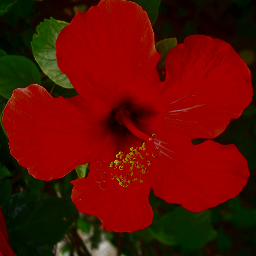
\includegraphics[width=.15\linewidth]{section4-constrast-6}\\
$\gamma=0{,}5$&$0{,}75$&$1$&$1{,}5$&$2$&$3$
\end{tabular}}{Modifier une image en couleur par une transformation de puissance de son intensité moyenne.}{fig-contrast-color}

\section{Images et matrices}
\subsection{Transposition et rotation}
Écrivons une image comme une matrice $A=(a_{i,j})\in\mathbb{R}^{n\times p}$. Les lignes sont indexées de haut en bas par $1\leq i\leq n$, les colonnes de gauche à droite par $1\leq j\leq p$. La transposée $B=A^{\mathsf T}\in\mathbb{R}^{p\times n}$ vérifie
\[
 b_{j,i}=a_{i,j}.
\]
Elle échange les deux directions de coordonnées et réfléchit l'image par rapport à la direction diagonale. Un quart de tour dans le sens des aiguilles d'une montre produit une autre matrice $C$ de taille $p\times n$, définie par
\[
 c_{j,i}=a_{n-i+1,j},\qquad 1\leq j\leq p,\quad1\leq i\leq n.
\]
Autrement dit, le pixel initial $(i,j)$ se déplace en $(j,n-i+1)$. Ces opérations permutent les valeurs des pixels sans perdre d'information. Pour une image en couleur, on applique la même permutation à tous les canaux.
\myfigure{\imageTri{section10-original}{section10-transpose}{section10-rotation}{$A$}{$A^{\mathsf T}$}{Rotation horaire}}
{Transposition et rotation d'un quart de tour.}{fig-geometric}

\subsection{Fondu entre deux images}
Pour deux images $A$ et $B$ de mêmes dimensions et de même format de canaux, on définit
\[
 C_t=(1-t)A+tB,\qquad 0\leq t\leq1.
\]
Cette formule s'applique à chaque pixel et à chaque canal. Aux extrémités, $C_0=A$ et $C_1=B$ ; les valeurs intermédiaires produisent un \emph{fondu}. Comme les poids sont positifs et de somme un, les valeurs restent dans $[0,255]$ avant arrondi. Cette opération mélange les couleurs à positions fixes ; elle ne déplace pas les objets d'une position à une autre.
\myfigure{\begin{tabular}{@{}c@{\hspace{1mm}}c@{\hspace{1mm}}c@{\hspace{1mm}}c@{\hspace{1mm}}c@{\hspace{1mm}}c@{}}
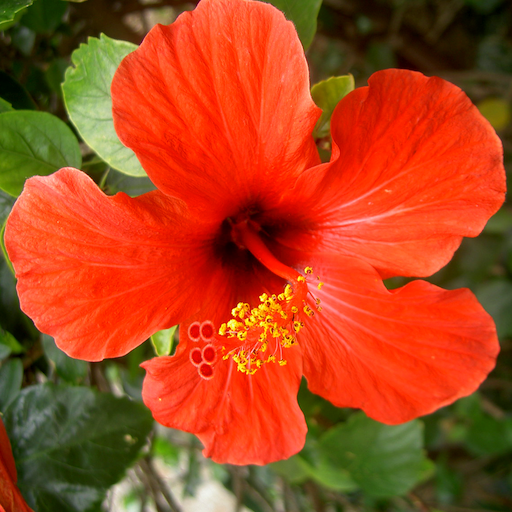
\includegraphics[width=.15\linewidth]{section11-interp-1}&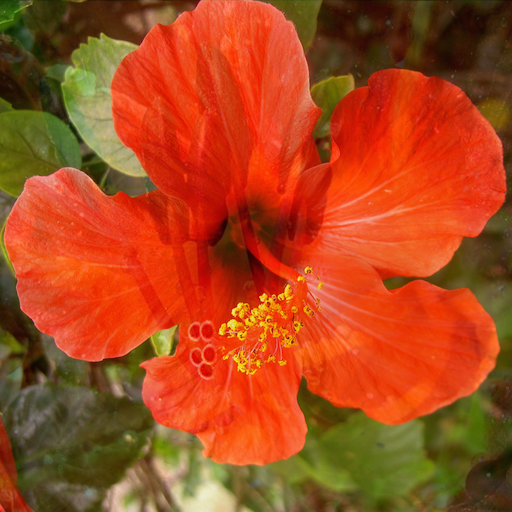
\includegraphics[width=.15\linewidth]{section11-interp-2}&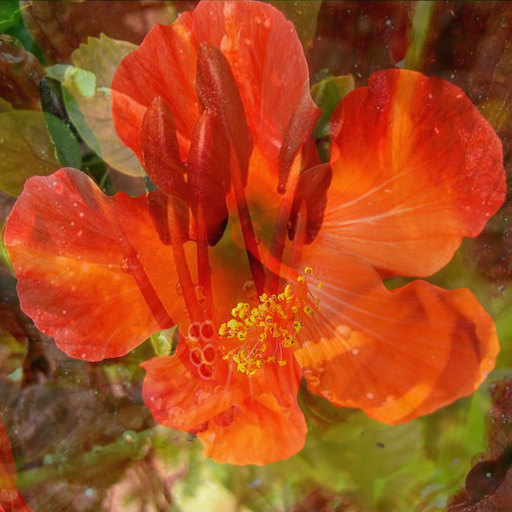
\includegraphics[width=.15\linewidth]{section11-interp-3}&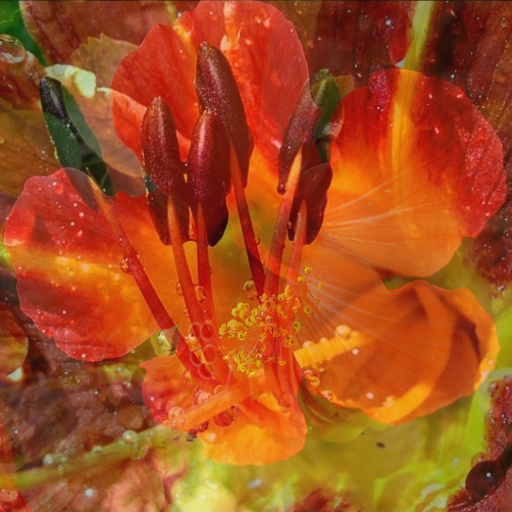
\includegraphics[width=.15\linewidth]{section11-interp-4}&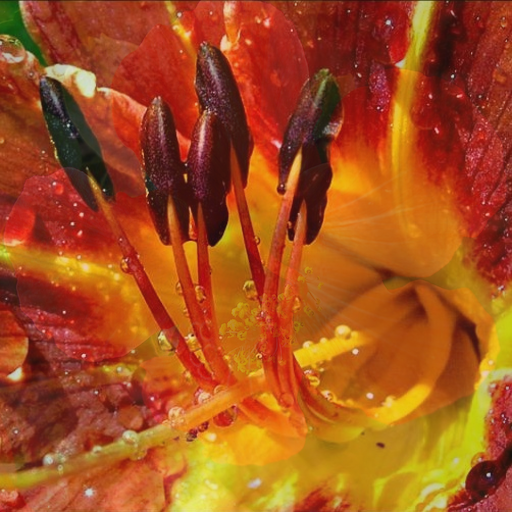
\includegraphics[width=.15\linewidth]{section11-interp-5}&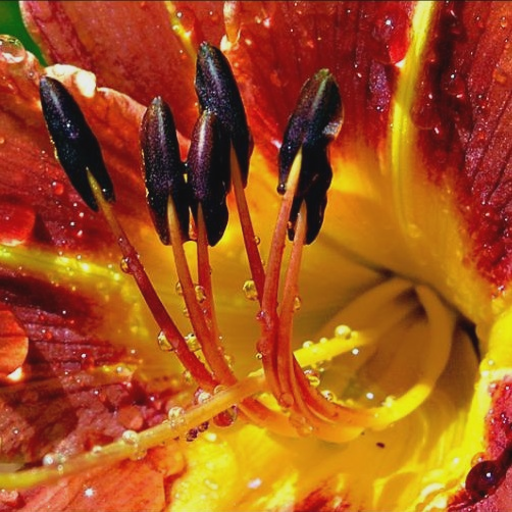
\includegraphics[width=.15\linewidth]{section11-interp-6}\\
$t=0$&$0{,}2$&$0{,}4$&$0{,}6$&$0{,}8$&$1$
\end{tabular}}{Interpolation linéaire de l'image $A$ vers l'image $B$.}{fig-interp}

\paragraph*{Pour aller plus loin.}
Les \href{https://www.numerical-tours.com/}{Numerical Tours}~\cite{2011-peyre-cise} proposent des expériences reproductibles. Ce chapitre reprend en partie l'article de l'auteur \emph{Le traitement numérique des images}, paru dans \emph{Images des mathématiques}.

\ifdefined\StandaloneChapter
\par\noindent\begin{minipage}{\linewidth}
\section*{Glossaire}
\begin{multicols}{2}\small\raggedright
\begin{rs}
\gloss{Bit et octet} : un chiffre binaire ; un groupe de huit bits.
\gloss{Pixel} : une case du tableau qui représente l'image.
\gloss{Canal} : l'un des tableaux de composantes d'une image multicanal.
\gloss{Quantification} : remplacement des valeurs par des indices d'un ensemble fini.
\gloss{Bruit} : fluctuations indésirables dues à l'acquisition ou au traitement.
\gloss{Moyenne} : somme des valeurs divisée par leur nombre.
\gloss{Médiane} : valeur centrale après classement d'un nombre impair de valeurs.
\gloss{Contour} : variation spatiale rapide des valeurs de l'image.
\gloss{Flou} : perte de transitions nettes et de détails fins.
\gloss{Contraste} : différences entre les régions claires et les régions sombres.
\gloss{Luminance} : grandeur photométrique définie à partir de la sensibilité visuelle.
\gloss{Matrice} : tableau rectangulaire $(a_{i,j})$.
\gloss{Résolution} : terme qui peut désigner les dimensions en pixels ou le pouvoir de séparation spatial ; ce sont deux notions distinctes.
\gloss{Fondu} : moyenne pondérée de deux images à positions de pixels fixes.
\end{rs}
\end{multicols}
\end{minipage}\par
\fi
